\documentclass[article,twoside]{dennou777}
\pagestyle{Dnofoot}

\ltjsetparameter{jacharrange={-2}}%ギリシア文字、キリル文字を AL Char に。
\usepackage[no-math,match,deluxe,fontspec,jfm_yoko=jlreq,jfm_tate=jlreqv]{luatexja-preset}

\usepackage[T1]{fontenc}
\usepackage{yhmath,amsmath,mathtools,amssymb,mathrsfs,rsfso,mleftright}
\usepackage[math]{kurier}
\usepackage[euler-digits]{eulervm}
\usepackage[scaled]{beramono}
%\usepackage{classico,newpxtext}
\DeclareMathAlphabet{\mathtt}{T1}{fvm}{m}{n}
\DeclareMathAlphabet{\mathsf}{T1}{uop}{m}{n}

\usepackage[unicode,colorlinks]{hyperref}
% \hypersetup{linkcolor=blue,urlcolor=teal,citecolor=olive}
\hypersetup{linkcolor=black,urlcolor=black,citecolor=black}

\usepackage{pxrubrica}
\usepackage{autobreak}
\usepackage{tcolorbox}
\usepackage{epmaketitle} %https://github.com/matryo-sika/epmaketitle
\renewcommand{\maketitle}{\epmaketitle}

\setmainfont{Exo 2}
\setsansfont{Exo 2}
\setmainjfont{FOT-MatissePro-DB}[
	AltFont={
		{
			Range={
				"4E00-"9FFF, % CJK 統合漢字
				"3400-"4DFF, % CJK 統合漢字拡張 A
				"20000-"2EBE0, % CJK 統合漢字拡張 B-F
				"2460-"24FF, % 囲み英数字
				"3200-"32FF, % 囲み CJK 文字・月
				"1F100-"1F2FF % 囲み英数字補助、漢字補助
			},
			Font=FOT-RodinNTLGPro-DB,
		},
	},
	BoldFeatures={
		Font=FOT-MatissePro-EB,
		AltFont={
			 {
				Range={
					"4E00-"9FFF, % CJK 統合漢字
					"3400-"4DFF, % CJK 統合漢字拡張 A
					"20000-"2EBE0, % CJK 統合漢字拡張 B-F
					"2460-"24FF, % 囲み英数字
					"3200-"32FF, % 囲み CJK 文字・月
					"1F100-"1F2FF % 囲み英数字補助、漢字補助
				},
				Font=FOT-RodinNTLGPro-EB,
			},
		},
	},
	YokoFeatures={JFM=jlreq},   % jlreqのJFMを維持する
	TateFeatures={JFM=jlreqv},  % https://qiita.com/zr_tex8r/items/91ae1dcc9c3afce7fa8c
]
\setsansjfont{FOT-RodinNTLGPro-DB}[
	AltFont={
		{
			Range={
				"4E00-"9FFF, % CJK 統合漢字
				"3400-"4DFF, % CJK 統合漢字拡張 A
				"20000-"2EBE0, % CJK 統合漢字拡張 B-F
				"2460-"24FF, % 囲み英数字
				"3200-"32FF, % 囲み CJK 文字・月
				"1F100-"1F2FF % 囲み英数字補助、漢字補助
			},
			Font=FOT-RodinNTLGPro-DB,
		},
	},
	BoldFeatures={
		Font=FOT-MatissePro-EB,
		AltFont={
			 {
				Range={
					"4E00-"9FFF, % CJK 統合漢字
					"3400-"4DFF, % CJK 統合漢字拡張 A
					"20000-"2EBE0, % CJK 統合漢字拡張 B-F
					"2460-"24FF, % 囲み英数字
					"3200-"32FF, % 囲み CJK 文字・月
					"1F100-"1F2FF % 囲み英数字補助、漢字補助
				},
				Font=FOT-RodinNTLGPro-EB,
			},
		},
	},
	YokoFeatures={JFM=jlreq},   % jlreqのJFMを維持する
	TateFeatures={JFM=jlreqv},  % https://qiita.com/zr_tex8r/items/91ae1dcc9c3afce7fa8c
]\setmonofont[
	Ligatures=TeX,
	Scale=0.89,
]{DejaVu Sans Mono}
\setmonojfont[
	Ligatures=TeX,
	Scale=0.89,
]{NotoSansMonoCJKjp-Regular}

\allowdisplaybreaks[4]
\ltjenableadjust[lineend=extended,priority=true,profile=true,linestep=true]

%%%%%%%%%%%%自作マクロ

%%matrix
\newcommand{\Mtx}[1]{\begin{matrix} #1 \end{matrix}}
\newcommand{\pMtx}[1]{\begin{pmatrix} #1 \end{pmatrix}}
\newcommand{\bMtx}[1]{\begin{bmatrix} #1 \end{bmatrix}}
\newcommand{\BMtx}[1]{\begin{Bmatrix} #1 \end{Bmatrix}}
\newcommand{\vMtx}[1]{\begin{vmatrix} #1 \end{vmatrix}}
\newcommand{\VMtx}[1]{\begin{Vmatrix} #1 \end{Vmatrix}}

\newcommand{\hmvec}{\mathbold}
\newcommand{\eqdef}{\stackrel{\mathrm{def}}{=}}
\newcommand{\centeralign}[1]{\rule{0pt}{0pt}\hfill#1\hfill\rule{0pt}{0pt}}
\newcommand{\Unit}[1]{\,\mathrm{#1}}
\newcommand{\hmemph}[1]{\textbf{#1}}

\renewcommand{\thefootnote}{*\arabic{footnote}}

\Dtitle[大気放射の基礎]{大気放射の基礎\\--Liou著 藤枝・深堀訳 (2014) の講読--}
\Dauthor{人見祥磨}
\studentid{02160611}
\faculty{北海道大学理学部地球惑星科学科\\惑星宇宙グループ}
\advisor{石渡正樹}

\begin{document}

\begin{titlepage}
	\maketitle
\end{titlepage}

\cleardoublepage

\rule{0pt}{0pt}\vfill
\section*{要旨}
ハドレー循環について勉強するにつれて、惑星大気の熱輸送について興味を持った。
地球でない惑星における大気の熱輸送のふるまいは自転周期や地軸の傾きによって
大きく変化すると期待される。

そこで惑星大気の熱輸送についてシュミレーションをするために、大気の温度分布を
知る必要がある。そのためには、大気の放射フラックス密度を計算しなければならない。
大気の放射フラックス密度を計算するために、まずは放射に関する基本的な物理量を
導入する。そして、放射が流れることで、放射の強度が増減することを記述する
放射伝達方程式を導く。

実際に大気の温度分布を知るためには、微分方程式で表される放射伝達方程式を解かなければ
ならない。そのために、放射伝達方程式を形式的に解き、さらに具体的に数値解を求める
手法として、相関 $k$ 分布法について紹介する。
\vfill\rule{0pt}{0pt}

\pagebreak

\tableofcontents
\pagebreak

\section{動機}

ゼミでハドレー循環について勉強するにつれて、惑星大気の熱輸送について興味を持った。
ハドレー循環とは、赤道で大気が加熱され上昇して高緯度へ移動した後に、下降して地表
付近を南下して赤道へ戻るという、大気の大循環のことである。地球でない惑星についても、
ハドレー循環が起こりうると考えられ、そのふるまいは自転周期や地軸の傾きによって大きく
変化すると期待される。

そこで、惑星大気について、自転周期や地軸の傾きによって、どのように熱輸送が変化する
シミュレーションしたいと思った。そのためには大気の温度分布を計算する必要がある。
その計算をするために、放射に関して、観測なども含めて基礎事項を解説している Liou
の教科書~\cite{liou} を講読し、基礎的な事項について確認することとした。

\section{放射とは}

\hmemph{放射}とは電磁波の総称であり、輻射とも呼ばれる\cite{asano}。放射は、大気中の
エネルギー輸送を担う重要な過程であり、波動の形で伝搬する。そして、全ての放射は同じ速さ、
すなわち光速$c=2.9979\times10^8\Unit{m/s}$ で伝播する。

電磁波では、周波数 $\tilde\nu$ と波長 $\lambda$ が以下の式で関連付けられる。
\begin{equation}
	\lambda=\frac{c}{\tilde\nu}
\end{equation}
また、赤外放射の特性を表すために、習慣的に以下の式で表される波数 $\nu$ も用いられる。
\begin{equation}
	\nu=\frac{\tilde\nu}{c}=\frac{1}{\lambda}
\end{equation}

\section{基本的な放射量}

放射が流れることで、放射は相互作用により増減する。これを記述する
\hmemph{放射伝達方程式}を導く。そのために、放射量を表すための物理量を定義する。

\begin{figure}[t]
	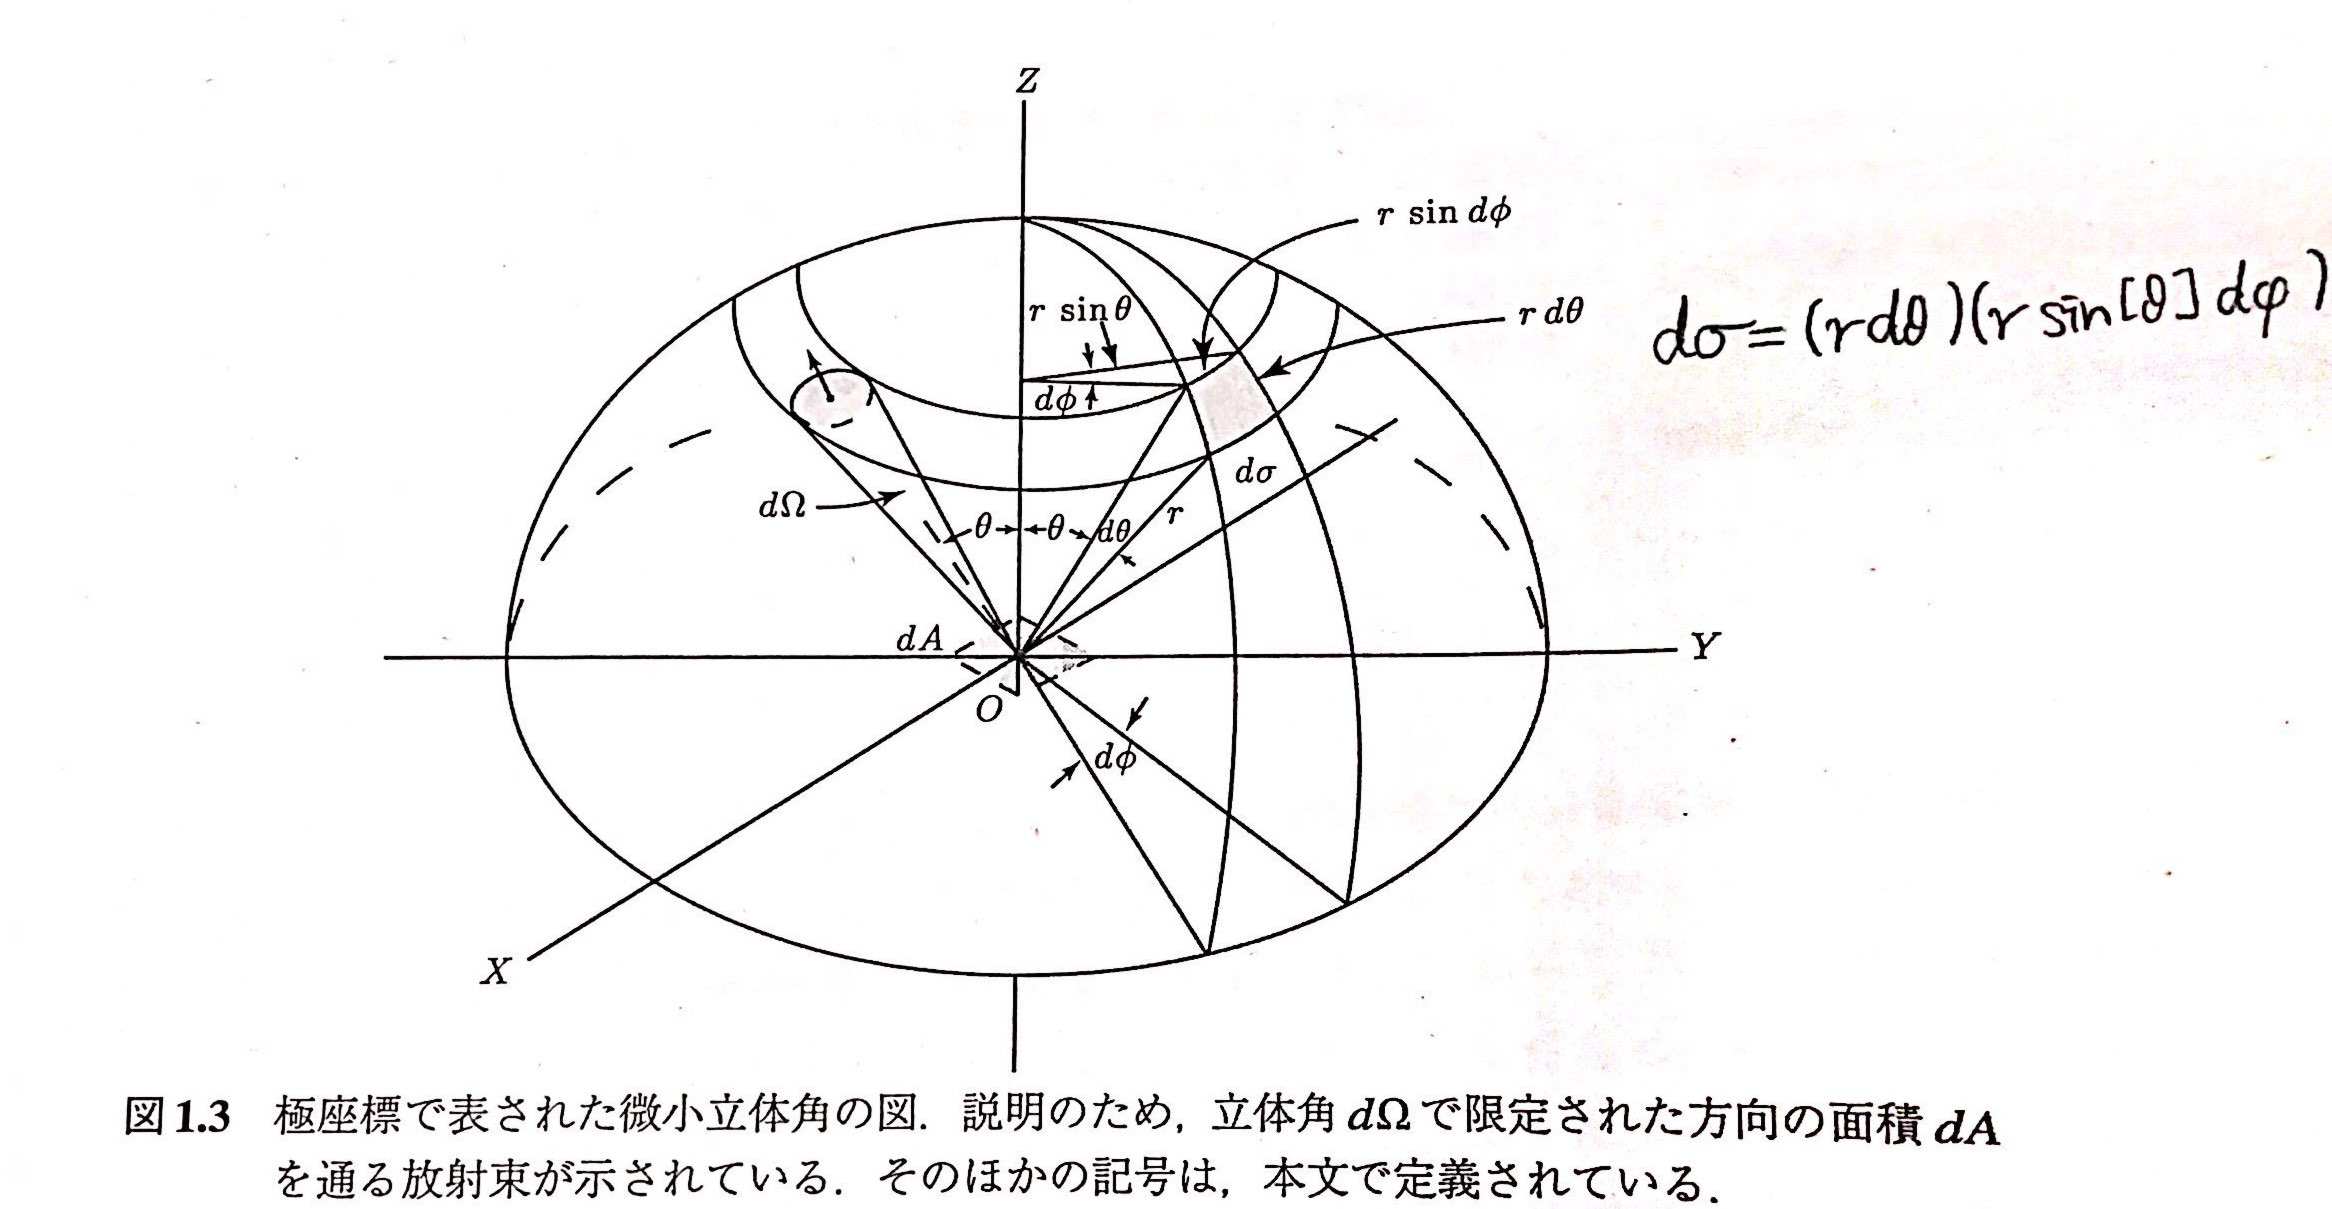
\includegraphics[width=\linewidth]{eq.jpg}
	\caption
		[極座標で示された微小立体角の図]
		{極座標で示された微小立体角の図。Liou~\cite{liou} による。}
\end{figure}

\hmemph{単色の放射強度} $I_\lambda$ を導入する。
面積 $dA$ を横切り、$dA$ の法線からなす角 $\theta$ の方向にある微小立体角 $d\Omega$
から入射する、ある波長区間 $\lambda$ 〜 $\lambda+d\lambda$ における、微小時間 $dt$
の間の微小放射エネルギー量 $dE_\lambda$ を考える。このとき、$dE_\lambda$ は単色の
放射強度$I_\lambda$ に関する式として、
\begin{equation}
	dE_\lambda=I_\lambda\cos[\theta]\,dA\,d\Omega\,d\lambda\,dt
\end{equation}
で表されるとする。すなわち、単色の放射強度は以下の式で定義される。
\begin{equation}
	I_\lambda=\frac{dE_\lambda}{\cos[\theta]\,dA\,d\Omega\,d\lambda\,dt}
\end{equation}
式より明らかなように、単色の放射強度には、放射が流れる方向が含まれている。

半球の全立体角にわたって積分された $I_\lambda$ の法線成分は、
\hmemph{単色の放射フラックス密度} $F_\lambda$ と呼ばれる。
\begin{equation}
	F_\lambda=\int_\Omega I_\lambda\cos[\theta]\,d\Omega
\end{equation}
特に、等方性放射、すなわち放射強度が方向に依存しない場合は、単色の放射フラックス密度は
\begin{equation}
	F_\lambda=\pi I_\lambda
\end{equation}
となる。

\hmemph{全放射フラックス密度} $F$ は単色の放射フラックス密度を、波長全体で積分したものである。
\begin{equation}
	F=\int^\infty_0 F_\lambda\,d\lambda
\end{equation}
全放射フラックス密度を、面全体で積分したものは\hmemph{全放射フラックス} $f$ と呼ばれる。
\begin{equation}
	f=\int_AF\,dA
\end{equation}

\begin{table}[t]
	\caption{様々な放射量の記号、次元、及び単位}
	\centering
	\begin{tabular}{clll}
		\hline
		記号&放射量&次元&単位\\
		\hline\hline
		$E$&放射エネルギー&$\Unit{ML^2T{-2}}$&$\Unit{J}$\\
		$f$&放射フラックス&$\Unit{ML^2T{-3}}$&$\Unit{J\,s^{-1}}$, $\Unit{W}$\\
		$F$&放射フラックス密度&$\Unit{MT^{-3}}$&$\Unit{W\,m^{-2}}$\\
		$I$&放射強度&$\Unit{MT^{-3}}$&$\Unit{W\,m^{-2}\,sr^{-2}}$\\
		\hline
	\end{tabular}
\end{table}

\section{散乱と吸収の概念}
放射伝達方程式を考えるためには、放射が流れるにあたって、その過程でどのように
放射が変化するかを考えなければならない。具体的には、
放射は散乱や吸収という過程を経て、強度が変化する。
このことは、放射伝達方程式に記述するために、実際にどのような現象が発生しているか確認する。

入射波と衝突した粒子が、入射した電磁波のエネルギーを、あらゆる方向に
再放射する過程は\hmemph{散乱}と呼ばれる。散乱はすべての波長で発生し、粒子の大きさが影響する。
粒子の大きさが散乱に及ぼす影響は、サイズパラメーター $x=2\pi a/\lambda$ ($a$ は粒径)に
よって推定することができる。また、散乱は
粒子が少ないとき、個々の粒子が全く同じように散乱する\hmemph{独立散乱}と、
粒子が多量にあるとき、散乱が繰り返される\hmemph{多重散乱}に分けられる。

\begin{figure}[t]
	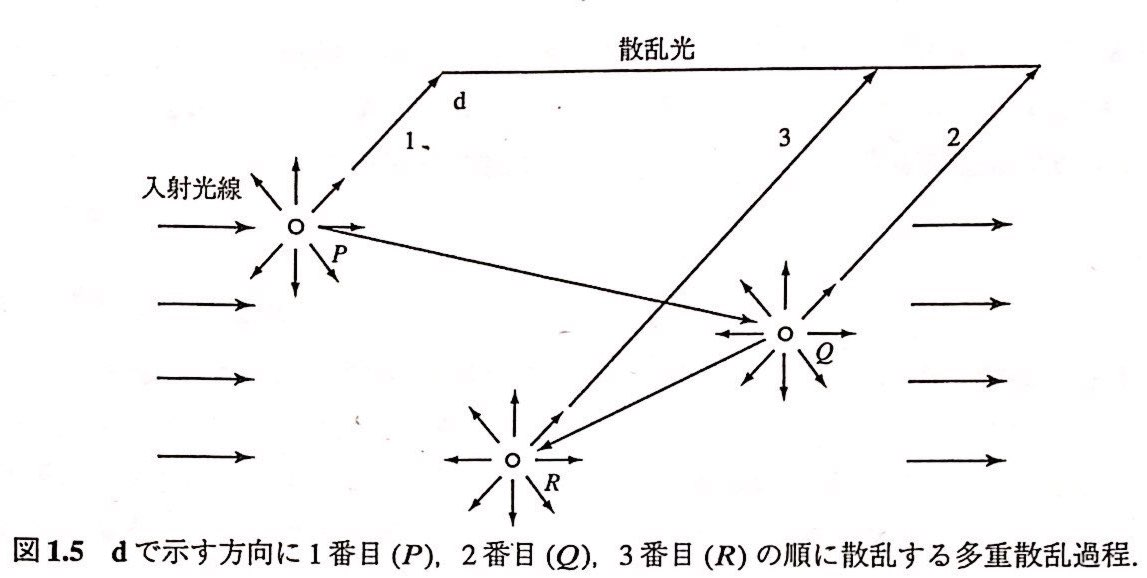
\includegraphics[width=\linewidth]{mscatter.jpg}
	\caption
		[多重散乱過程を示す図]
		{$\mathrm{d}$ で示す方向へと散乱する、多重散乱過程。Liou~\cite{liou} より。}
\end{figure}
\begin{figure}[t]
	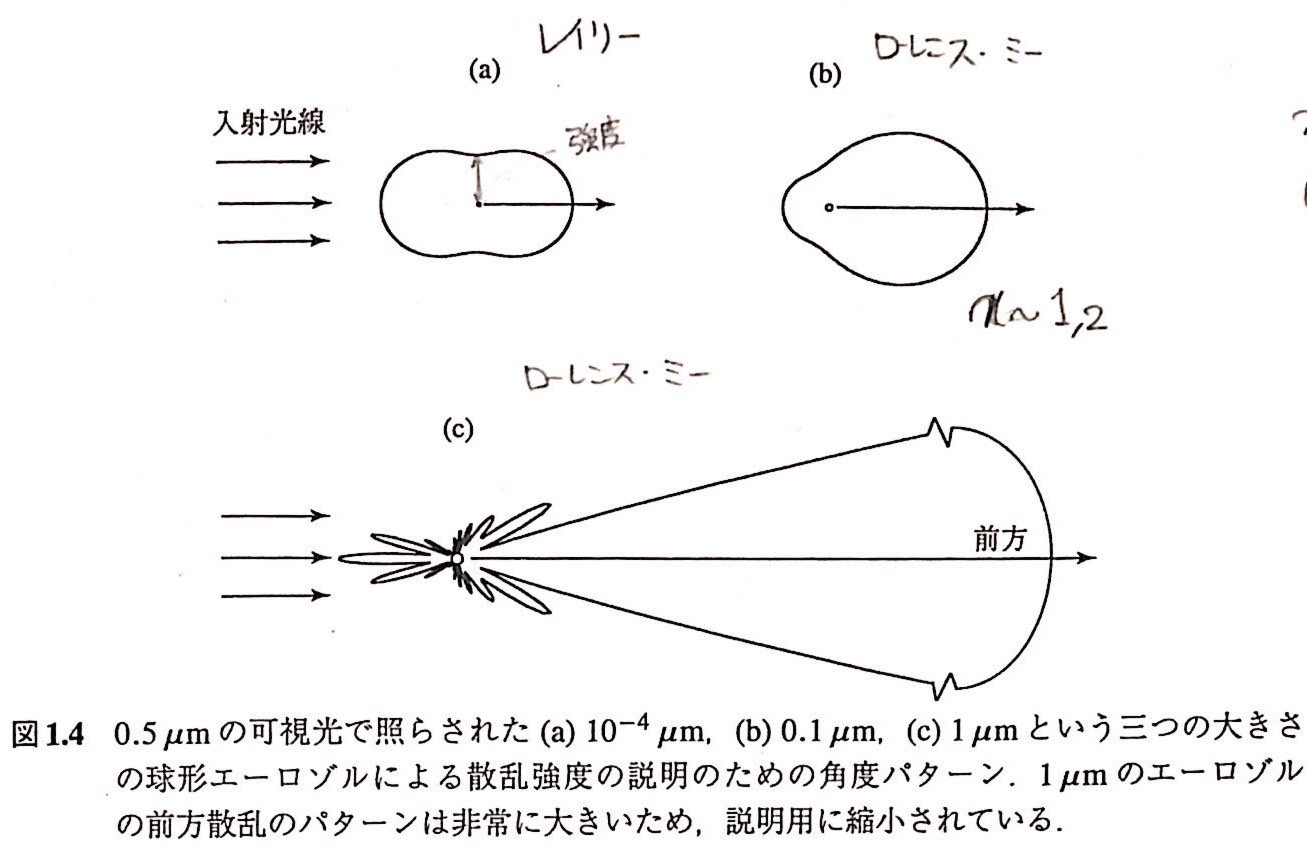
\includegraphics[width=0.8\textwidth]{scatter.jpg}
	\caption
		[サイズパラメーターが散乱へ及ぼす影響]
		{サイズパラメーター $x$ の、散乱に及ぼす影響を示した図。Liou~\cite{liou}より。}
\end{figure}

\section{黒体放射の法則}

\hmemph{黒体}とは吸収のない理想的な物体である。
放射を考える上で、最も基本的な物体として黒体を考える。
これより、黒体の放射を支配する 4 つの法則について述べる。

\subsection{プランクの法則}
プランク (Planck, 1901) は、原子が黒体表面に小さな電磁振動子のような振る舞いをしていると
仮定し、振動子が持つエネルギーが
\begin{equation}
	E=nh\tilde\nu
\end{equation}
に量子化されると仮定した。ここで、$n\in\mathbb{Z}$ は量子数、$h$ はプランク定数、
$\tilde\nu$ は振動子の周波数である。

放出されたエネルギーを求めるためには、マクスウェル・ボルツマン統計に従った、起こりうる
全ての状態の周波数 $\tilde\nu$ から振動子の総数を知る必要がある。以上の仮定をもとに、
振動子あたりの平均放射エネルギーで正規化すると、射出された単色の放射強度を表す式として、
周波数と絶対温度の関数であるプランク関数が次のように求まる\footnote{プランク関数の導出は
付録にて行う}。
\begin{equation}
	B_{\tilde{\nu}}[T]=\frac{2h\tilde{\nu}^3}{c^2(\exp[h\tilde{\nu}/k_\mathrm{B}T]-1)}
\end{equation}
ここで、$h$ はプランク定数、 $k_\mathrm{B}$ はボルツマン定数、$c$ は光速、$T$ は絶対温度
である。プランク定数とボルツマン定数は実験によって決定され、
$h=6.626\times10^{-34}\Unit{J\,s}$、$K_\mathrm{B}=1.3806\times10^{-23}\Unit{J\,K^{-1}}$
である。さらに、波長 $\lambda=c/\tilde\nu$ に関する式に書き直すと、
\begin{equation}
	B_\lambda[T]=\frac{2hc^2}{\lambda^5(\exp[hc/k_\mathrm{B}\lambda T]-1}=
	\frac{C_1\lambda^{-5}}{\pi(\exp[C_2/\lambda T]-1)}
\end{equation}
を得る。ここで、$C_1=2\pi hc^2$、$C_2=hc/k_\mathrm{B}$ である。

\begin{figure}[t]
	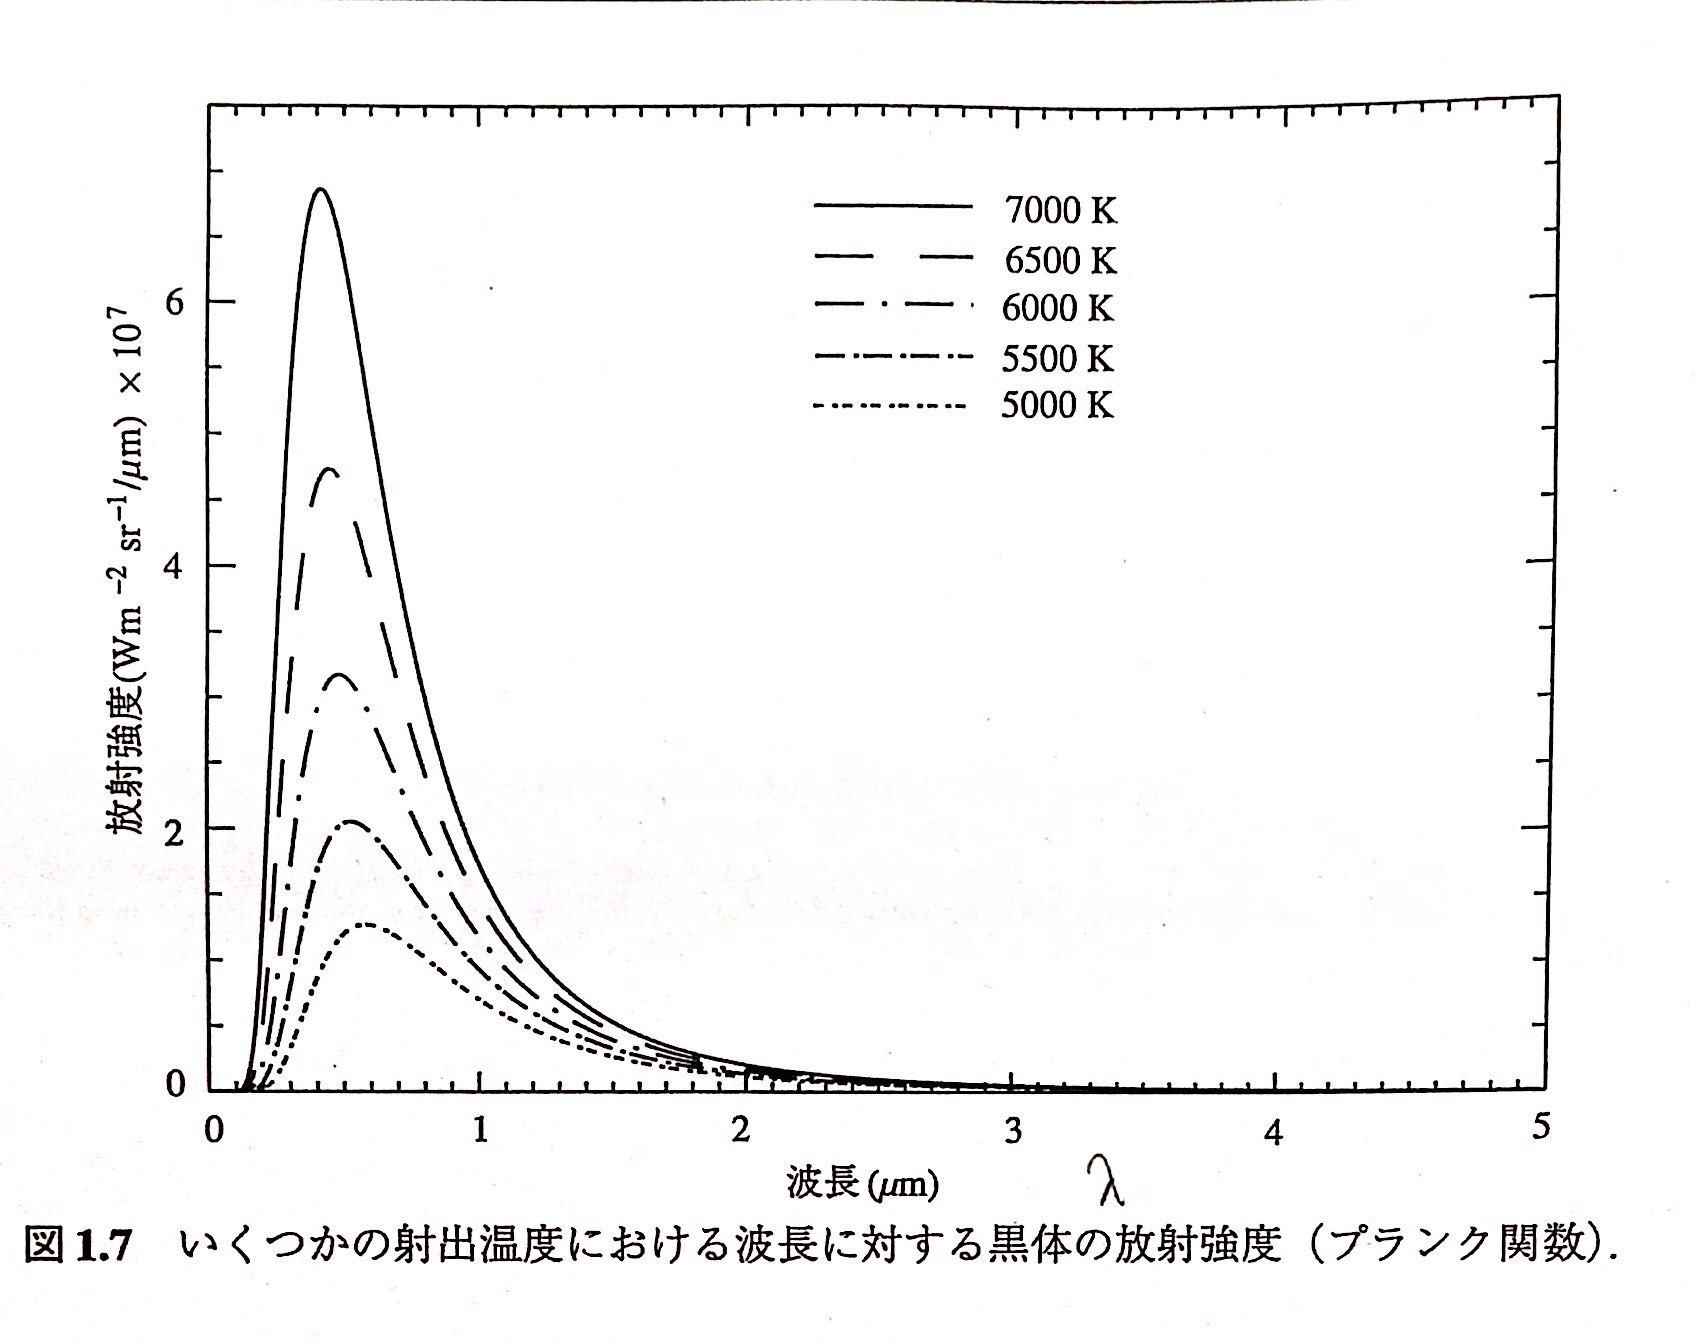
\includegraphics[width=\textwidth]{planck.jpg}
	\caption
		[プランク関数]
		{
			いくつかの射出温度における、波長に対する黒体の放射強度(プランク関数)。
			Liou~\cite{liou}より。
		}
\end{figure}

\subsection{ステファン・ボルツマンの法則}
黒体の全放射強度を求めるためには、プランク関数を波長全体で積分すればよい。ここで、
$b=2\pi^4k_\mathrm{B}^4/(15c^2h^3)$ を導入すると、
\begin{equation}
	B[T]=\int^\infty_0 B_\lambda[T]\,d\lambda=bT^4
\end{equation}
と求められる。さらに、等方な黒体によって放射される放射フラックス密度を求めると、
\begin{equation}
	F=\pi B[T]=\sigma T^4
\end{equation}
となる。ここで、$\sigma=5.67\times10^{-8}\Unit{J\,m^{-2}\,s^{-1}\,k_\mathrm{B}^{-4}}$は
ステファン・ボルツマン定数と呼ばれる。

この式は、黒体によって放出される放射フラックス密度が、絶対温度の $4$ 乗に比例することを
示していて、\hmemph{ステファン・ボルツマンの法則}と呼ばれる。これは、広い波長域での
赤外放射伝達の解析をする際に基礎となる法則である。

\subsection{ウィーンの変位則}
黒体放射の最大放射強度の波長が、温度に反比例することを、\hmemph{ウィーンの変位則}と呼ぶ。

黒体放射の最大放射強度の波長を求めるには、プランク関数を波長で偏微分し、その偏微分係数が
$0$ になる波長を求めれば良い。
\begin{equation}
	\frac{\partial B_\lambda[T]}{\partial\lambda}=0
\end{equation}
これを解くと
\begin{equation}
	\lambda_m=\frac{a}{T}
\end{equation}
を得る。ここで、$a=2.897\times10^{-3}\Unit{m\,K}$ はウィーンの変位定数と呼ばれている。

\subsection{キルヒホッフの法則}
\hmemph{キルヒホッフの法則}は、射出と吸収が等しくなるという法則である。
キルヒホッフの法則が成り立つためには、以下の条件を満たしていなければならない。
すなわち、温度が一様であり、等方性放射が達成される、熱力学的平衡の条件が必要である。

この条件は、中間圏よりも高度が低い局所的に限られた空間で、
分子の衝突によってエネルギー遷移が起こる範囲内ならば、精度良く成り立つと考えることができる。

\section{スペクトル線の広がり}
単色の放射は、原子や分子への外部からの影響と、射出の際のエネルギー損失のため、
エネルギー遷移する間にエネルギー準位が僅かに変化する。
その結果、非単色の放射となり、有限の幅を持つスペクトル線が観測される

\subsection{ローレンツ線形}
分子や原子の衝突によって広げられたスペクトル線の線形をローレンツ線形と呼ぶ。

ローレンツ線形は
\begin{equation}
	k_\nu=\frac{S}{\pi}\frac{\alpha}{(\nu-\nu_0)^2+\alpha^2}=Sf[\nu-\nu_0]
\end{equation}
によって定式化される。ここで、$k_\nu$は吸収係数、$\nu_0$ は理想的な単色の吸収線の波数、
$\alpha$ は吸収線の半値半幅であり、圧力と温度の関数、$f$ は形状因子 (shape factor);\quad
$\displaystyle S=\int^\infty_{-\infty}k_\nu\,d\nu$: 線強度

\begin{figure}[t]
	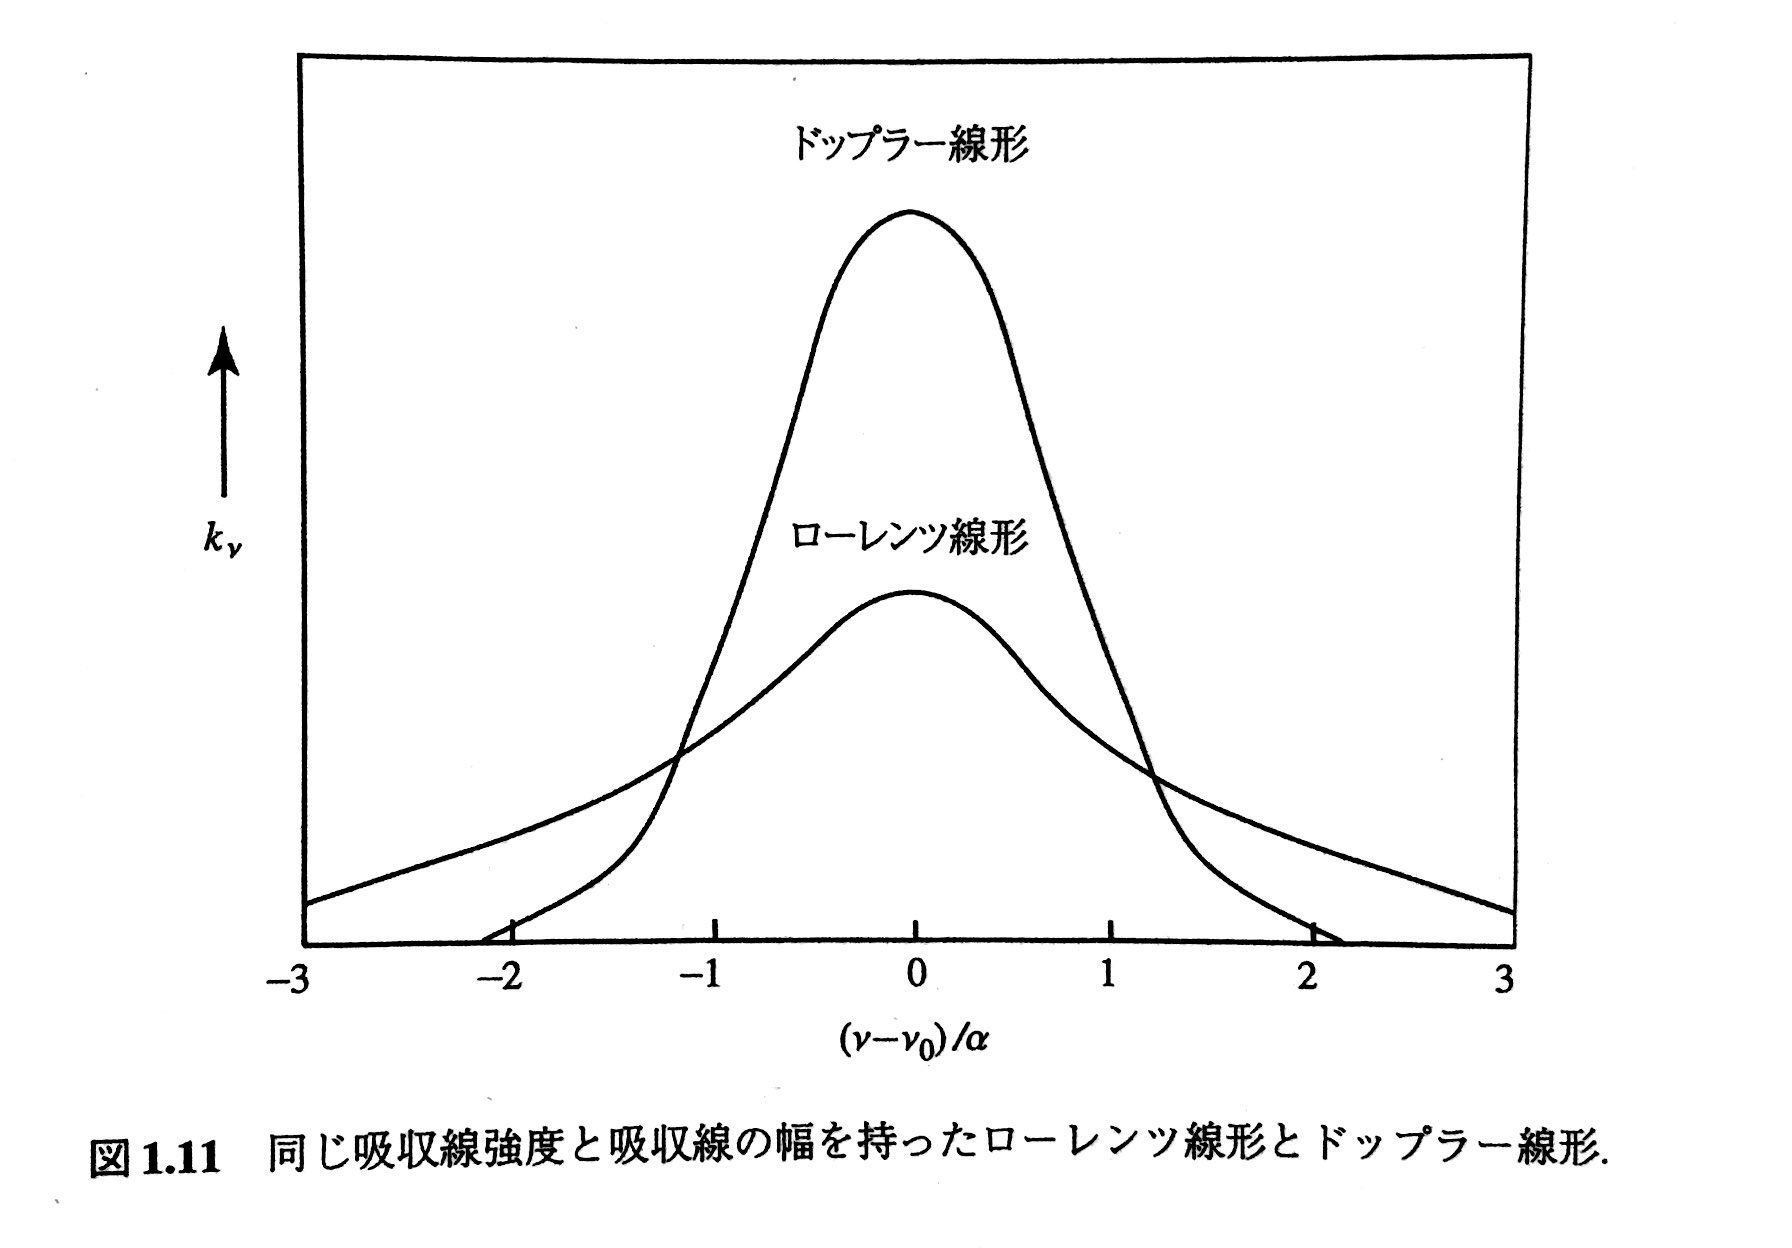
\includegraphics[width=\textwidth]{lorentz.jpg}
	\caption
		[ローレンツ線形とドップラー線形]
		{
			同じ吸収線強度と吸収線の幅を持った、ローレンツ線形とドップラー線形。
			Liou~\cite{liou} より。
		}
\end{figure}


\section{放射伝達方程式の導出}
ある方向に進む放射が、吸収や散乱などの相互作用で、どのように増減するか記述するのが、
放射伝達方程式である。放射伝達方程式を導き、特定の状況での放射伝達方程式の解を求める。

まず、放射伝達強度の変化 $dI_\lambda$ を、物質との相互作用による減少
$dI_\lambda^\mathrm{d}$ と、射出と多重散乱による増加 $dI_\lambda^\mathrm{s}$ に分けて考える。
\begin{equation}
	dI_\lambda=dI_\lambda^\mathrm{d}+dI_\lambda^\mathrm{s}
\end{equation}

$dI_\lambda^\mathrm{d}$ について、放射の伝搬方向に厚さ $ds$ で密度 $\rho$ の媒質を
横切った後に、放射強度が減少したとする。このとき、
\begin{equation}
	dI_\lambda^\mathrm{d}=-k_\lambda\rho i_\lambda\,ds
\end{equation}
となる。ここで、係数 $k_\lambda$ は質量消散断面積と呼ばれる。

一方で、以下の式によって放射源係数 $j_\lambda$ を導入して、放射伝達強度の増加
$dI_\lambda^\mathrm{s}$ を
\begin{equation}
	dI_\lambda^\mathrm{s}=j_\lambda\rho\,ds
\end{equation}
で表す。

以上の式より
\begin{equation}
	dI_\lambda=dI_\lambda^\mathrm{d}+dI_\lambda^\mathrm{s}
	=-k_\lambda\rho I_\lambda\,ds+j_\lambda\rho\,ds
\end{equation}
を得る。さらに、放射源関数 $J_\lambda\equiv j_\lambda/k_\lambda$ を導入すると、
\begin{equation}
	\frac{dI_\lambda}{k_\lambda\rho\,ds}=-I_\lambda+J_\lambda
\end{equation}
となる。これが\hmemph{放射伝達方程式}である。

\subsection{ビーアー・ブーゲー・ランバートの法則}
ここからは、具体的な場合の放射伝達方程式の解を考える。

大気系からの射出の寄与を無視できる場合を考えよう。この場合は、放射源関数 $J_\lambda$
が無視できるので、放射伝達方程式は
\begin{equation}
	\frac{dI_\lambda}{k_\lambda\rho\,ds}=-I_\lambda
\end{equation}
となる。$s=0$ における入射強度を $I_\lambda[0]$ とし、距離 $s_1$ 離れた位置における
射出強度 $I_\lambda[s_1]$ を求めるために、これを積分すると
\begin{equation}
	I_\lambda[s_1]=I_\lambda[0]\exp[-\int^{s_1}_0 k_\lambda\rho\,ds]
\end{equation}
となる。ここで、媒質が均一であると仮定すると、$k_\lambda$ は $s$ に依存しないので、光路長を
\begin{equation}
	u=\int^{s_1}_0\rho\,ds
\end{equation}
として定義すると、
\begin{equation}
	I_\lambda[s_1]=I_\lambda[0]\exp[-k_\lambda u]
\end{equation}
を得る。

この結果は、一様に消散する媒質を横切る放射強度の低下が、質量消散断面積と光路長の積の
指数関数に従うことを示していて、\hmemph{ビーアー・ブーゲー・ランバートの法則}と呼ばれている。


\subsection{シュワルツシルトの方程式}
地球と大気から射出される熱赤外放射伝達について考える。
このとき、放射源関数はプランク関数で与えられる。
この場合の放射伝達方程式は、シュワルツシルトの式と呼ばれる。
\begin{equation}
	\frac{dI_\lambda}{k_\lambda\rho\,ds}=-I_\lambda+B_\lambda[T]
\end{equation}

シュワルツシルトの式の解は、$s$ と $s_1$ の間の光学的厚さ
\begin{equation}
	\tau_\lambda[s_1,s]=\int^{s_1}_s k_\lambda\rho\,ds
\end{equation}
を定義することによって、
\begin{equation}
	I_\lambda[s_1]=I_\lambda[0]\exp\bigl[-\tau_\lambda[s_1,0]\bigr]+
	\int^{s_1}_{0}B_\lambda\bigl[T[s]\bigr]\exp\bigl[-\tau_\lambda[s_1,s]\bigr]k_\lambda\rho\,ds
\end{equation}
で与えられる\footnote{この式の導出は付録にて行う}。


\section{大気の熱赤外放射伝達}
放射伝達方程式から、大気の放射フラックス密度を形式的に得よう。
そのために、放射強度は時間に依存しないと仮定し、大気は平衡平面であり、
放射強度と大気パラメーターは鉛直方向にのみ変化すると仮定する。

放射強度と大気パラメーターは鉛直方向にのみ変化するので、放射強度は天頂角と鉛直位置のみの
関数である。放射源関数として、プランク放射強度 $B_\nu[z]=B_\nu[T[z]]$ を用いると、
高度座標の放射伝達方程式は
\begin{equation}
	-\mu\frac{dI_\nu[z,\mu]}{k_\nu\rho_a\,dz}=I_\nu[z,\mu]-B_\nu[z]
\end{equation}
となる。

この式には、$dz$、$k_\nu$、$\rho_a$の積が含まれているので、次の式で与えられる光学的深さ
$\tau$ を導入すると便利である。ここで、$\mathrm{TOA}$ は大気上端であり、
$p=\rho_a/\rho$ は気体の混合比である。
\begin{equation}
	\tau=\int^{\mathrm{TOA}}_{z} k_\nu[z]\rho_a[z]\,dz=\int^p_0 k_\nu[p]q[p]\frac{dp}{g}
\end{equation}
この式より、光学的深さの微分は次のようになる。
\begin{equation}
	d\tau=-k_\nu[z]\rho_a[z]\,dz=k_\nu[p]q[p]dp/g
\end{equation}
ここで、放射伝達方程式を $\tau$ 座標に変換すると、
\begin{equation}
	\mu\frac{dI_\nu[\tau,\mu]}{d\tau}=I_\nu[\tau,\mu]-B_\nu[\tau]
\end{equation}
を得る。

これは 1 階微分方程式であるから、全光学的厚さ $\tau_*$ である大気の、
上向き成分と下向き成分を解くためには、適切に境界条件を設定しなければならない。
そこで、地球表面からの射出と大気上端 (TOA) からの射出が等方性となると仮定する。

一般に、地球表面は赤外の領域では黒体と仮定できるので、$I_\nu[\tau_*,\mu]=B_\nu[\tau_*]$
となる。さらに、大気上端では下向きの放射源がなく、 $I_\nu[0,-\mu]=B[\mathrm{TOA}]\simeq0$
であるとと仮定する。この境界条件に従うと、上向きと下向きの放射強度は、
\begin{align}
	I^\uparrow_\nu[\tau,\mu]
		&=B_\nu[\tau_*]e^{-\tau_*=\tau)/\mu}
		+\int^{\tau_*}_\tau B_\nu[\tau']e^{-\tau_*=\tau)/\mu}\frac{d\tau'}{d\mu}\\
	I^\downarrow_\nu[\tau,-\mu]
		&=\int^{\tau_*}_\tau B_\nu[\tau']e^{-\tau_*=\tau)/\mu}\frac{d\tau'}{d\mu}
\end{align}
で与えられる。この解に含まれる、指数関数的な減衰を表すことができるように、単色の透過率
$T_\nu[\tau/\mu]=e^{-\tau/\mu}$ を定義すると、放射強度の型式解は
\begin{align}
	I^\uparrow_\nu[\tau,\mu]
		&=B_\nu[\tau_*]T_\nu\left[\frac{\tau_\nu-\tau}{\mu}\right]
		-\int^{\tau_*}_\tau B_\nu[\tau']\frac{d}{d\tau'}T_\nu\left[\frac{\tau'-\tau}{\mu}\right]d\tau'\\
	I^\downarrow_\nu[\tau,-\mu]
		&=\int^\tau_0 B_\nu[\tau']\frac{d}{d\tau'}T_\nu\left[\frac{\tau-\tau'}{\mu}\right]d\tau'
\end{align}
で表すことができる。

大気の加熱率の計算に必要な放射フラックス密度は、上半球と下半球の放射強度の和であるから、
\begin{equation}
	F^{\uparrow\downarrow}_\nu[\tau]=2\pi\int^1_0 I^{\uparrow\downarrow}_\nu[\tau,\pm\mu]\mu\,d\mu
\end{equation}
である。角度方向の積分を考慮するため、拡散透過率
\begin{equation}
	T^f_\nu[\tau]=2\int^1_0 T_\nu\left[\frac{\tau}{\mu}\right]\mu\,d\mu
\end{equation}
を導入すると、放射フラックス密度は
\begin{align}
	F^\uparrow_\nu[\tau]
		&=\pi B_\nu[\tau_*]T^f_\nu[\tau_*-\tau]
		-\int^{\tau_*}_\tau \pi B_\nu[\tau']\frac{d}{d\tau'}T^f_\nu[\tau'-\tau]d\tau'\\
	F^\downarrow_\nu[\tau]
		&=\int^\tau_0 \pi B_\nu[\tau']\frac{d}{d\tau'}T^f_\nu[\tau-\tau']d\tau'
\end{align}
で表される。放射フラックスの波数積分は、$\tau$ が波数の関数なので、
\begin{equation}
	F^{\uparrow\downarrow}[z]=\int^\infty_0 F^{\uparrow\downarrow}_\nu[z]\,d\nu
\end{equation}
となる。この表式からわかるように、全放射フラックスを得るためには、光学的深さに沿った
波数積分を必ず行わなければならない。

\subsection{分光透過率}
赤外放射伝達の計算をする際は、プランク関数の変動が無視しうるような
小さな波数区間で放射パラメーターを決めることが有効である。
放射強度と放射フラックスの方程式における基本的な放射パラメーターとして、
平均波数の添字 $\bar\nu$ のついた分光透過率を定義する。
\begin{equation}
	T_{\bar\nu}[u]
	=\int_{\Delta\nu}\exp[-\tau]\frac{d\nu}{\Delta\nu}
	=\int_{\Delta\nu}\exp\left[-\int_u\sum_j k_{\nu,j}[u]\,du\right]\frac{d\nu}{\Delta\nu}
\end{equation}

\section{相関 $k$ 分布法}
相関 $k$ 分布法は、赤外放射伝達を計算するための手法である。
均質な大気では分光透過率は吸収係数 $k$ の順序に依存しないので、波数積分は $k$ 空間での
積分に置き換えることができる。相関 $k$ 分布法は、気体の分光透過率を吸収係数 $k_\nu$ に
応じてグループとして扱い、積分空間を置換する手法である。

\begin{figure}[t]
	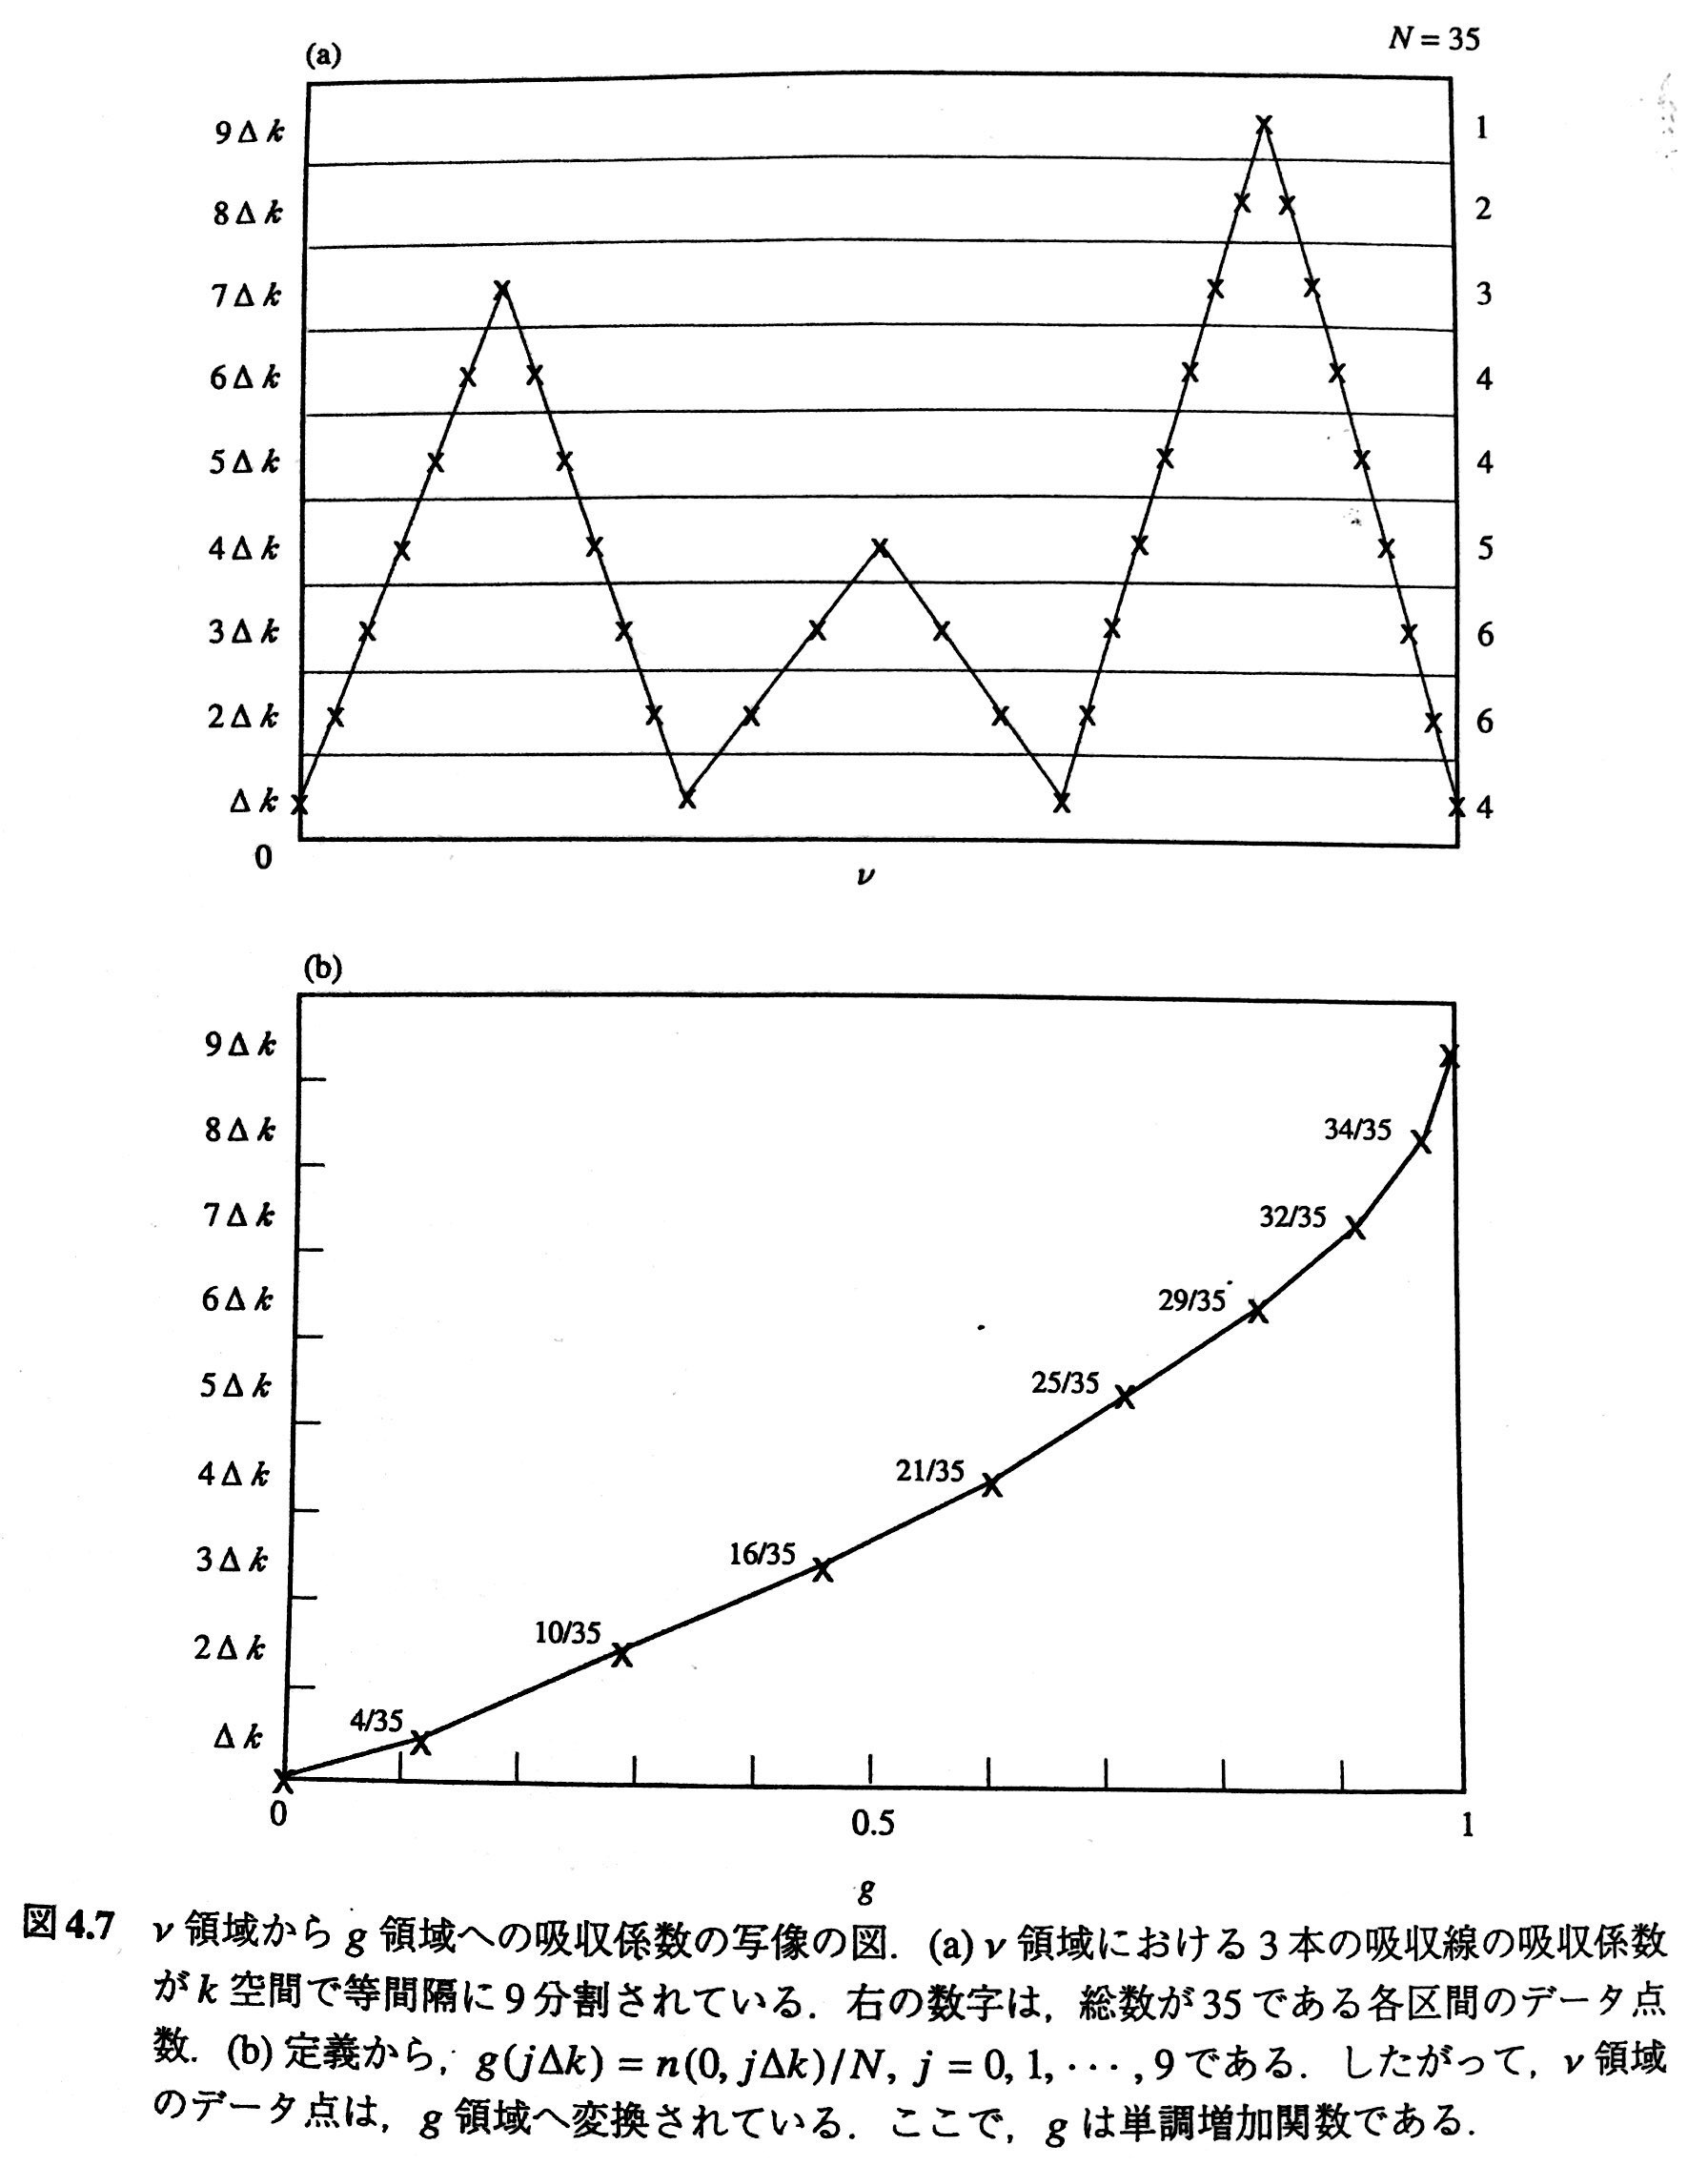
\includegraphics[width=\textwidth]{kbunpu.jpg}
	\caption
		[$\nu$ 空間から $g$ 空間への写像]
		{
			$\nu$ 空間から $g$ 空間へ置換する例。$\nu$ 空間から $g$ 空間へ置換することで
			和を取らなければならない点の数が減少している。Liou~\cite{liou}より。
		}
\end{figure}

波数区間 $\Delta\nu$ における $k_\nu$ に対する正規化確率密度関数が
$f[k]$ で与えられ、その最大値と最小値がそれぞれ $k_{\mathrm{min}}\to0$、
$k_{\mathrm{max}}\to\infty$ だとすると、分光透過率は
\begin{equation}
	T_{\bar\nu}[u]=\int_{\Delta\nu}\exp[-k_\nu u]\frac{d\nu}{\Delta\nu}
	=\int^\infty_0 \exp[-ku]f[k]\,dk
\end{equation}
で表すことができる。これより、確率密度関数 $f$ は分光透過率のラプラス逆変換であるとわかる。
\begin{equation}
	f[k]=\mathcal{L}^{-1}[T_{\bar\nu}[u]]
\end{equation}

さらに、累積確率分布関数を定義する。
\begin{equation}
	g[k]=\int^k_0 f[k]\,dk
\end{equation}
$g[0]=0$、$g[k\to\infty]=1$、$dg=f\,dk$ であるから、分光透過率は次で表すことができる。
\begin{equation}
	T_{\bar\nu}[u]=\int^1_0 \exp[-k[g]u]\,dg\simeq\sum_j\exp[-k[g_j]u]\,\Delta g_j
\end{equation}
これにより、分光透過率の計算を、冗長な波数区間における積分から、$g$ 空間における積分に
置換し、指数項の有限和によって求めることができるようになった。

\subsection{不均質大気への応用}
今述べた相関 $k$ 分布法の理論は、$\nu$ 積分を $g$ 積分で置き換えるために、
吸収係数 $k$ が一定であると仮定していた。現実大気では、吸収係数は圧力に応じて変化するので、
鉛直方向の吸収係数の変化を考えなければならない。すなわち、吸収係数が一定であると仮定して
導かれた 2 つの積分が、鉛直方向に吸収係数が変化しても等価であるかを評価しなければならない。
\begin{equation}
	T_{\bar\nu}[u]
	=\int_{\Delta\nu}\exp\left[-\int_u k_\nu\,du\right]\frac{d\nu}{\Delta\nu}
	\stackrel{?}{=}\int^1_0\exp\left[-\int_uk[g]\,du\right]dg
\end{equation}

最初に、波数区間 $-\Delta\nu/2$ から $\Delta\nu/2$ で単一の吸収線を考えよう。
吸収線の中心では $\nu[k_{\mathrm{max}}]=0$、吸収線の端では
$|\nu[k_{\mathrm{min}}]|=\Delta\nu/2$ となり、累積密度関数は以下になる。
\begin{equation}
	g[k]=\int^k_0 f[k]\,dk
	=\frac{2}{\Delta\nu}\int^k_{k_{\mathrm{min}}}\left|\frac{d\nu}{dk}\right|_{k=k'}dk'
	=\frac{2}{\Delta\nu}\nu[k]-1
\end{equation}
そして、$(2/\Delta\nu)\,d\nu=dg$となる。
すなわち、単一の吸収線の場合は $\nu$ 積分を $g$ 積分に置き換えることができる

次に、波数区間 $\Delta\nu$ 内で周期的に生起される吸収線を考える。
吸収線の間隔が $\delta$ であるとすると、
\begin{equation}
	g[k]=\int^k_0 f[k]\,dk
	=\frac{2}{\delta}\int^k_{k_{\mathrm{min}}}\left|\frac{d\nu}{dk}\right|_{k=k'}dk'
	=\frac{2}{\delta}\nu[k]-1
\end{equation}
そして、$(2/\Delta\nu)\,d\nu=dg$となる。
したがって、この場合も $\nu$ 積分を $g$ 積分に置き換えることができる

\section{まとめと今後の展望}

放射を考えるために必要な基本的な物理量を導入した上で、放射伝達方程式を導出した。
そして、大気系からの射出を無視できる場合や、シュワルツシルトの方程式といった特定の状況での
放射伝達方程式の解法や、放射強度の一般的な形式解を求めた。

そして、大気放射フラックス密度を実際に計算する方法について学んでいる。その手法の一つである
相関 $k$ 分布法は $\nu$ 積分を $g$ 積分に置換し、計算量を少なくすることができる手法である。
大気放射フラックス密度 $F$ が計算できると、$\partial F/\partial z$ より熱が収束する高度が
わかるので、温度分布を求めることができる。

現在は、相関 $k$ 分布法で計算をする手順を学んでいるので、実際に相関 $k$ 分布法を用いた計算を
行ってみたいと考えている。

\clearpage
\begin{thebibliography}{9}
	\bibitem{liou} 大気放射学 ---衛星リモートセンシングと気候問題へのアプローチ---
		K. N. Liou(著) 藤枝 鋼、深堀 正志(翻訳)
		共立出版 \textbf{(2014)}\quad672ページ
	\bibitem{asano} 大気放射学の基礎 浅野正二(著) 朝倉書店 \textbf{(2010)}\quad267ページ
\end{thebibliography}

\pagebreak
\listoffigures
\listoftables

\end{document}
